\subsection{Tracking downloads with different speeds}
In this synthetic experiment we measure if MultiChain can correctly track the upload and download amounts
between two peers with different speeds.
In this scenario a file of 100 MB is downloaded repeatedly at different speeds,
respectively 500 KB/s, 750 KB/s, 1000 KB/s, 1250 KB/s, 2000 KB/s, and 3000 KB/s.
The maximum speed of anonymous download was measured in experiments to be 1150 KB/s~\cite{ruigrok-anonymous}.
The upload and download of the file is done by different pairs of seeders and downloaders.

\begin{figure}
\centerline{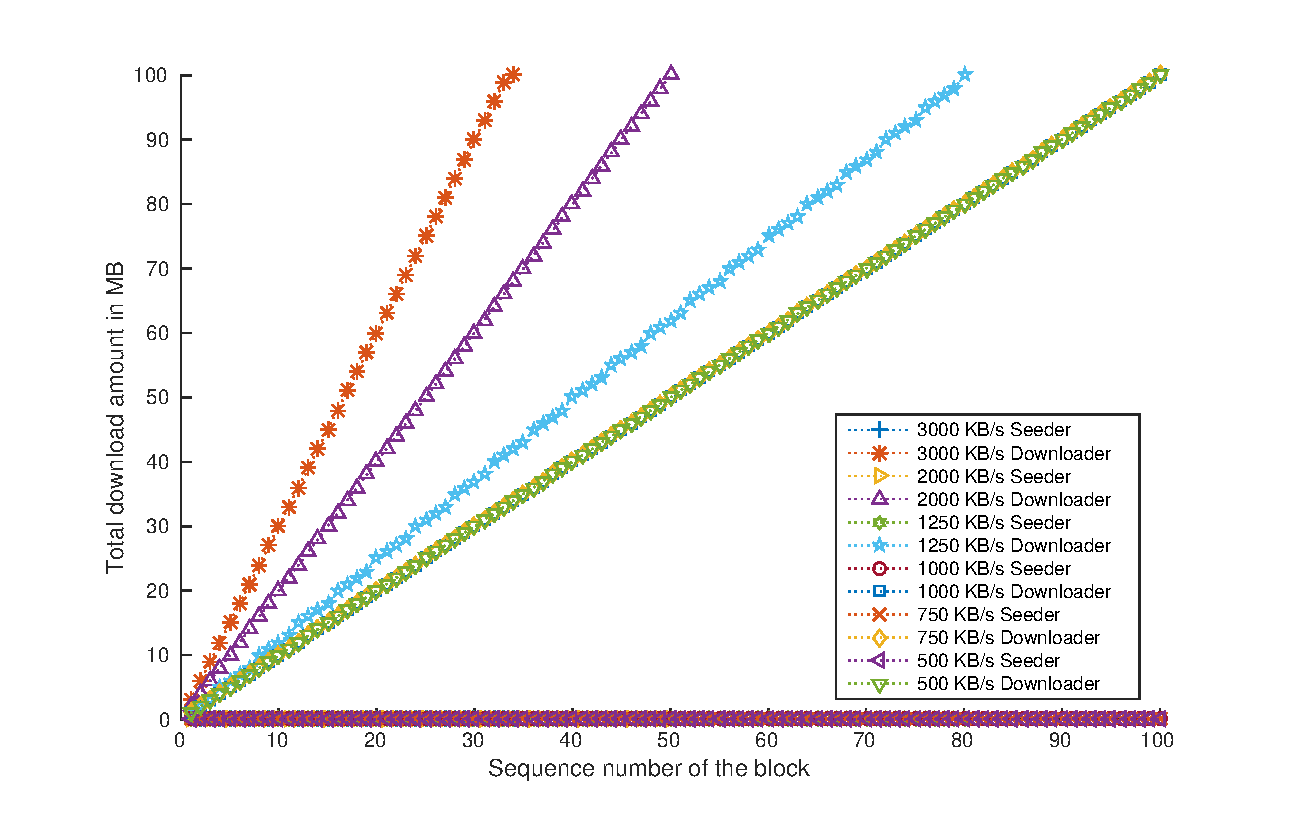
\includegraphics[scale=0.5]{experimentation/speeds/synthetic-simple-down.eps}}
\caption{Total download amounts repeated 6 times with different speeds.}
\label{fig:synthetic-simple-amounts}
\end{figure}

The total download amount of every downloader is plotted in Figure \ref{fig:synthetic-simple-amounts}.
These amounts are plotted in the same way as the previous experiment.
The upload amount of every seeder is identical to the amount of download of the corresponding downloader.
The plots show that MultiChain is able to correctly track the download and upload amounts without a problem.
The plots are smooth and the amounts go up in fixed increments corresponding to the different speeds.
Downloads at a a faster speed result in higher download amounts in the blocks.
This means that MultiChain is fast enough to correctly track the amounts.

The download speeds below the threshold of 1000 MB of the scheduler
are not distinguishable from the download at the threshold speed.
There are three overlapping lines.
We call this the scheduler effect.
This is because the scheduler waits until the threshold is reached before initiating the block.
The amount is tracked in the same amount of blocks,
but the total time of the experiment is longer for these experiments.
If the speed goes above the threshold, then this is reflected in the figure.
The blocks tracks amounts in whole units of MB,
this causes the download at 750 KB/s to not grow faster than the download at 500 KB/s.
Any leftover KBs are saved for the next block.

This experiment was run several times before the final version in this report was run.
Earlier versions of the experiment resulted in two bugfix and two improvements:
the ability of the scheduler to create a block at the end of a download.